\section{Introducción}\label{sec:1_introduccion}

Los objetos con alto desplazamiento al rojo o alto \rt \footnote{A lo largo del trabajo haremos referencia a objetos con un \rt\ alto, medio y bajo. La distinción típica que se encuentra en la literatura es: alto \rt\ \maths{z>1}, \rt\ intermedio \maths{0.1<z<1} y \rt\ bajo \maths{z<0.1}} en inglés, (en lo sucesivo utilizaremos el término \rt\ por brevedad) son muy importantes para entender cómo se formaron las estructuras que observamos en el universo actual. En su gran mayoría se trata de galaxias en estadios tempranos de su formación que se caracterizan por una magnitud aparente muy débil y una emisión electromagnética principalmente en la zona infrarroja (IR) del espectro. Debido a que la generación actual de telescopios infrarrojos (en especial aquellos que operan en el infrarrojo lejano, \microm{\lambda\sim100-500}) tienen una resolución espacial bastante limitada en comparación con los telescopios ópticos (la resolución angular de un telescopio con apertura circular es proporcional al inverso de su diámetro y los telescopios que operan en el \mbox{IR-lejano} deben ser telescopios espaciales pues la atmósfera es opaca en esa zona del espectro) las medidas realizadas sobre las galaxias tempranas en formación\footnote{También nos referiremos a estos objetos como \comillas{galaxias lejanas}, \comillas{galaxias submilimétricas} (en referencia al rango del espectro en el que son mas brillantes), o \comillas{galaxias tempranas}. Debe quedar claro que en este trabajo cuando utilizamos el término \comillas{galaxia temprana} nos referimos siempre a un orden cronológico y no a la morfología de la galaxia.} (\mbox{ETGs}) tienen una gran contaminación debido a la presencia de otras fuentes débiles en sus proximidades y son especialmente difíciles de estudiar. 

A veces, la luz procedente de los objetos lejanos resulta desviada debido a la presencia de objetos muy masivos que se interponen entre estas fuentes y nosotros (generalmente galaxias elípticas y grupos de galaxias) y se producen intensas magnificaciones (entendiéndose como un incremento sobre el brillo original) de la imagen del objeto fuente. Este fenómeno, conocido como lente gravitatoria, lejos de ser un problema está resultando ser una importante herramienta para el estudio de las propiedades individuales y estadísticas de las galaxias submilimétricas~(SMGs). Eso ha motivado la aparición de distintas propuestas para la identificación de galaxias lejanas lensadas\footnote{En las publicaciones realizadas en lengua inglesa, se refieren a estos objetos con el nombre de \comillas{\anglicismo{gravitationally lensed galaxies}}, sin embargo resulta difícil traducir correctamente esta terminología al castellano. A falta de una traducción mejor usaremos la palabra \comillas{lensar} en lugar del término \anglicismo{lensed}.} (SLGs) entre los cartografiados de galaxias actuales. En particular, los trabajos de \cite{article:Negrello_2010} y \cite{article:Nuevo_2012} proponen unos criterios para seleccionar este tipo de galaxias a partir de las medidas del telescopio espacial infrarrojo \h. Ambos criterios proponen la identificación de los candidatos a partir de la selección de distintos flujos de corte para un conjunto de frecuencias consideradas. Estos métodos, como cualquier otro, tienen sus propios sesgos de selección, por lo que resultaría interesante disponer de otros métodos radicalmente diferentes para seleccionar SLGs.

En este trabajo planteamos la búsqueda de SLGs  identificando sistemas lente gravitatoria completos, es decir, encontrando no solo el objeto fuente que ha sido lensado, sino también el objeto lente cuya masa es responsable de la desviación de la luz procedente de la fuente. Al igual que los autores anteriores, nosotros proponemos la búsqueda de SLGs en el catálogo \hatlas\ porque es sensible a las longitudes de onda en el IR-lejano en el que se produce el máximo de emisión de las ETGs y porque se ha estimado que la sección eficaz de detección de lentes a alto \rt\ por el instrumento \spire\ es muy favorable \citep{article:Negrello_2010}. En este caso, debido a que existe una zona de solapamiento entre los cartografiados \hatlas\ y \gama\ y también debido a que la distribución en \rt\ de los objetos del catálogo \gama\ es la adecuada, consideramos el catálogo \gama\ como una buena elección para encontrar en él los objetos lente. Nuestra idea consiste en aplicar un criterio estadístico de \cross\ de catálogos de galaxias para identificar lentes gravitatorias en las que participa como objeto fuente una \etg. El método consta de dos factores de Bayes propuestos por \cite{article:Tamas_Budavari_2008} y  \cite{article:Tamas_Budavari_2011}; uno de ellos depende de la separación angular entre las observaciones\footnote{En este trabajo se entiende por observación al conjunto de dos medidas: posición y desplazamiento al rojo. Cada catálogo realiza sus propias observaciones de forma independiente.} y otro de la diferencia entre los \rt. Cada emparejado considerado está formado por dos observaciones, una de ellas perteneciente al catálogo \hatlas\ y la otra a \gama. En los casos en los que se cuenta con una medida fiable del corrimiento al rojo de la observación realizada por \hatlas\ se utilizarán esos valores; en caso de que no se disponga de dicha información, se realizará un ajuste por mínimos cuadrados de la distribución espectral de energía (\sed) de una galaxia modelo a tres medidas del flujo espectral en tres longitudes de onda diferentes realizadas por el instrumento \spire. Si el ajuste se considera adecuado proporcionará el \rt\ fotométrico de la fuente. En el caso de que el factor de Bayes conjunto dé una alta probabilidad de que el par de observaciones no pertenezcan a un mismo objeto, pero el término que depende de la distancia angular sugiere que si lo son, el par de observaciones es considerado un sistema lente gravitatoria.

La memoria está dividida en varias secciones: la Sección \ref{sec:1_introduccion} contiene una explicación básica de algunos de los conceptos más importantes que serán usados a lo largo del trabajo; la Sección \ref{sec:2_muestras} pretende dar una explicación general de los catálogos utilizados y de los instrumentos con los que se realizaron; la Sección \ref{sec:3_redshift_hatlas} describe el método utilizado en este trabajo para calcular el \rt\ fotométrico de las ETGs a partir de las medidas del instrumento \spire, se explicarán también los fundamentos en los que se basa y confrontaremos el \rt\ obtenido para un conjunto de  galaxias con los obtenidos por otros autores; en la Sección \ref{sec:4_cross_identificacion} describiremos en detalle el método de \cross\ utilizado; en la Sección \ref{sec:5_halos} se describirán las distintas propuestas para para identificar los sistemas que conforman lentes gravitatorias, incluida la nuestra; en la Sección \ref{sec:6_resultados} se mostrarán\linebreak los resultados obtenidos y finalmente, Sección \ref{sec:7_conclusiones}, expondremos nuestras conclusiones. Los apéndices contienen tablas y el código de los programas escritos en lenguaje de programación \python.


\subsection{Galaxias con alto desplazamiento al rojo.}\label{subsec:galaxias_alto_rojo}

Las galaxias con alto desplazamiento al rojo son galaxias muy lejanas, cuya luz ha tardado miles de millones de años en recorrer la distancia que nos separa de ellas y que ahora, vistas desde la Tierra, muestran el aspecto que tuvieron cuando la luz partió de ellas. Estos objetos juegan un papel fundamental en cosmología, porque su estudio permite comprender cómo se formaron las galaxias actuales.
Una de las predicciones fundamentales de la teoría del \anglicismo{Big Bang} es que el universo temprano consistía en materia y radiación distribuida de forma homogénea y en equilibrio termodinámico. Hoy día el universo es altamente heterogéneo, formando estructuras como estrellas, galaxias, cúmulos y supercúmulos de galaxias. Entender cómo se produjo esta etapa de transición entre el universo homogéneo a la formación de las estructuras que se observan en el universo actual, es uno de los objetivos de la cosmología y de la física fundamental.

\subsubsection{Características de las galaxias con alto desplazamiento al rojo.}

Se especula que las primeras galaxias, se formaron a partir de nubes de gas compuestas por hidrógeno y pequeñas cantidades de helio y litio. En estas condiciones se formaron un gran número de estrellas, en un periodo de tiempo relativamente corto, conocido como \anglicismo{starburst} (estallido estelar). Para una galaxia del tamaño de la Vía Láctea con \maths{\sim {10}^{11}} estrellas, se cree que el proceso duró \maths{\sim {10}^8\;\mathrm{yr}}, lo que implica una tasa de formación estelar (SFR) \tfe{\sim 10^3}, una cifra enorme si se compara con la tasa de formación estelar actual de la misma \tfe{\sim 1} \citep{book:encyclopedia}. Estas primeras estrellas, forman la primera generación de estrellas en el Universo, llamada Población III y tenían unas características distintas a las actuales. Se cree que eran muy masivas, llegando a poseer masas de hasta \masassolares{100}. Actualmente, las nebulosas donde se forman las nuevas estrellas contienen metales\footnote{ Se entiende por metales todos los núcleos atómicos con masa atómica superior al He. Estos elementos no se encontraban en el universo antes de la aparición de las primera estrellas.}, lo cual incrementa su opacidad; la radiación emitida durante el colapso de la nebulosa interacciona con el material y parte de él no pasa a formar la estrella, porque que es expulsado, lo cuál limita la masa de las estrellas actuales. Las estrellas muy masivas queman muy rápidamente su combustible nuclear (los modelos indican que una estrella como el Sol está en la secuencia principal \maths{\sim {10}^{10}} años, mientras que las estrellas masivas con \masassolares{>25} tienen una vida media de menos de \maths{7\times{10}^{6}} años, \citealt{book:encyclopedia}), y finalizan su vida como supernovas que expulsan grandes cantidades de residuos nucleares que enriquecen el medio interestelar con elementos pesados.

Las estrellas pertenecientes a estas primera etapas del Universo debieron ser grandes emisoras de luz y radiación ultravioleta (UV). Las grandes nubes de gas y polvo que se encontraban en las galaxias que las albergaban absorbían una parte esta radiación y la remitían en el IR. Las temperaturas de equilibrio térmico para esas nubes se encuentran el rango de \maths{10-100\;\mathrm{K}}, lo que da lugar la emisión IR en la región \maths{\lambda \sim 30-300\;\mu \mathrm{m}} \citep{book:encyclopedia}.
Los halos galácticos de las galaxias espirales actuales de tipo S\maths{a} están compuestos por poblaciones de estrellas viejas, con edades \maths{\gtrsim 8-9\; \mathrm{Gyr}} (lo que corresponde a \maths{z\gtrsim 1-1.5}, \citealt{article:Lapi_2011}), las cuales se formaron a partir de los residuos nucleares de las estrellas que las precedieron y conforman la llamada Población II; por tanto, las ETGs muestran desplazamientos al rojo \maths{z \gtrsim 1}. La radiación IR procedente de una nube de polvo y gas interestelar perteneciente a una galaxia con un desplazamiento al rojo \maths{z=1} debería encontrarse en la zona del espectro con \maths{\lambda \sim 60-600\;\mu \mathrm{m}} (estas cifras se obtienen fácilmente a partir de la Ecuación \ref{eq:z_general} y el rango de emisión de las nubes al que se ha hecho referencia anteriormente). Estos datos suponen un punto de partida para la búsqueda de ETGs a partir de su observación en la zona IR del espectro.

\subsection{Desplazamiento al rojo.}

El desplazamiento al rojo (o desplazamiento al azul) es el desplazamiento del espectro electromagnético de un objeto hacia longitudes de onda mayores (o más cortas) que puede deberse a movimientos cinemáticos entre el emisor y el receptor (\maths{z_{mov}}, efecto Doppler), a efectos gravitatorios (\maths{z_{grav}}) o a la expansión de la métrica del universo a grandes escalas (\maths{z_{H}}). Dado un desplazamiento al rojo \maths{z}, podemos descomponerlo como la suma

\begin{equation}\label{eq:z_descomposicion}
    z= {z}_{mov}+{z}_{grav}+{z}_{H},
\end{equation}

de las distintas contribuciones citadas anteriormente. La definición general de corrimiento al rojo, siempre válida, independientemente de la causa que lo originó, es

\begin{equation}\label{eq:z_general}
    z=\frac{\lambda_o-\lambda_e}{\lambda_e}=\frac{\lambda_o}{\lambda_e}-1,
\end{equation}

donde los subíndices hacen referencia a la longitud de onda emitida \maths{e} y observada \maths{o}.

\subsubsection{Desplazamiento al rojo cosmológico.}

Cuando se habla de desplazamiento al rojo en el contexto de la cosmología, nos estamos refiriendo al hecho de que la distribución espectral de energía de las galaxias lejanas se encuentra desplazada hacia longitudes de onda mayores.  
Este hecho fue observado ya en el siglo XIX por aquellos que comenzaron a identificar líneas espectrales en los espectros emisión de los cuerpos celestes que en aquel momento se conocían como nebulosas\footnote{En aquel momento se conocían como nebulosas todos aquellos cuerpos celestes cuya luz no parecía provenir de una fuente puntual y su apariencia era similar a una nube de luz difusa. No estaba todavía establecida la diferencia entre nebulosas y galaxias.}.  Entre 1912 y 1925 el astrónomo italiano Vesto Sliper midió la posición de las líneas de emisión de unas 40 de estas nebulosas y constató por primer vez y para su sorpresa que, en todas ellas, las líneas se encontraban desplazadas hacia longitudes de onda inferiores con respecto a las mismas líneas espectrales medidas en el laboratorio \citep{book:cosmologia}. 
Posteriormente Edwin Hubble y su ayudante Milton Humanson, que disponían del mejor telescopio construido hasta entonces en el monte Palomar, Arizona, dieron un paso más en la comprensión del fenómeno. En primer lugar extendieron la lista elaborada por Sliper y probaron que en ningún caso el espectro se encontraba desplazado hacia el azul. En segundo lugar, Hubble identificó estrellas variables cefeidas en varios de estos cuerpos nebulosos\footnote{Fueron precisamente estudios como los que llevó a cabo Hubble para determinar las distancias, los que pusieron en evidencia que las galaxias y las nebulosas son objetos muy diferentes.} y gracias a ello pudo medir por primera vez la distancia a esos objetos. Interpretó el desplazamiento al rojo como un efecto Doppler y halló su velocidad a partir de la expresión

\vspace{-5mm}

\begin{equation}
    v\approx c z,
\end{equation}

e hizo una representación gráfica de la velocidad asociada a ese desplazamiento al rojo frente a la distancia que el midió. Se dio cuenta de que había una relación lineal entre la velocidad que y la distancia,

\begin{equation}
    v={H}_{0}D \implies z= ({H}_{0}/c)D.
\end{equation}

Ésta última igualdad es conocida como la ley de Hubble y \maths{{H}_0} como constante de Hubble.

\begin{figure}[htb]
    \begin{center}
         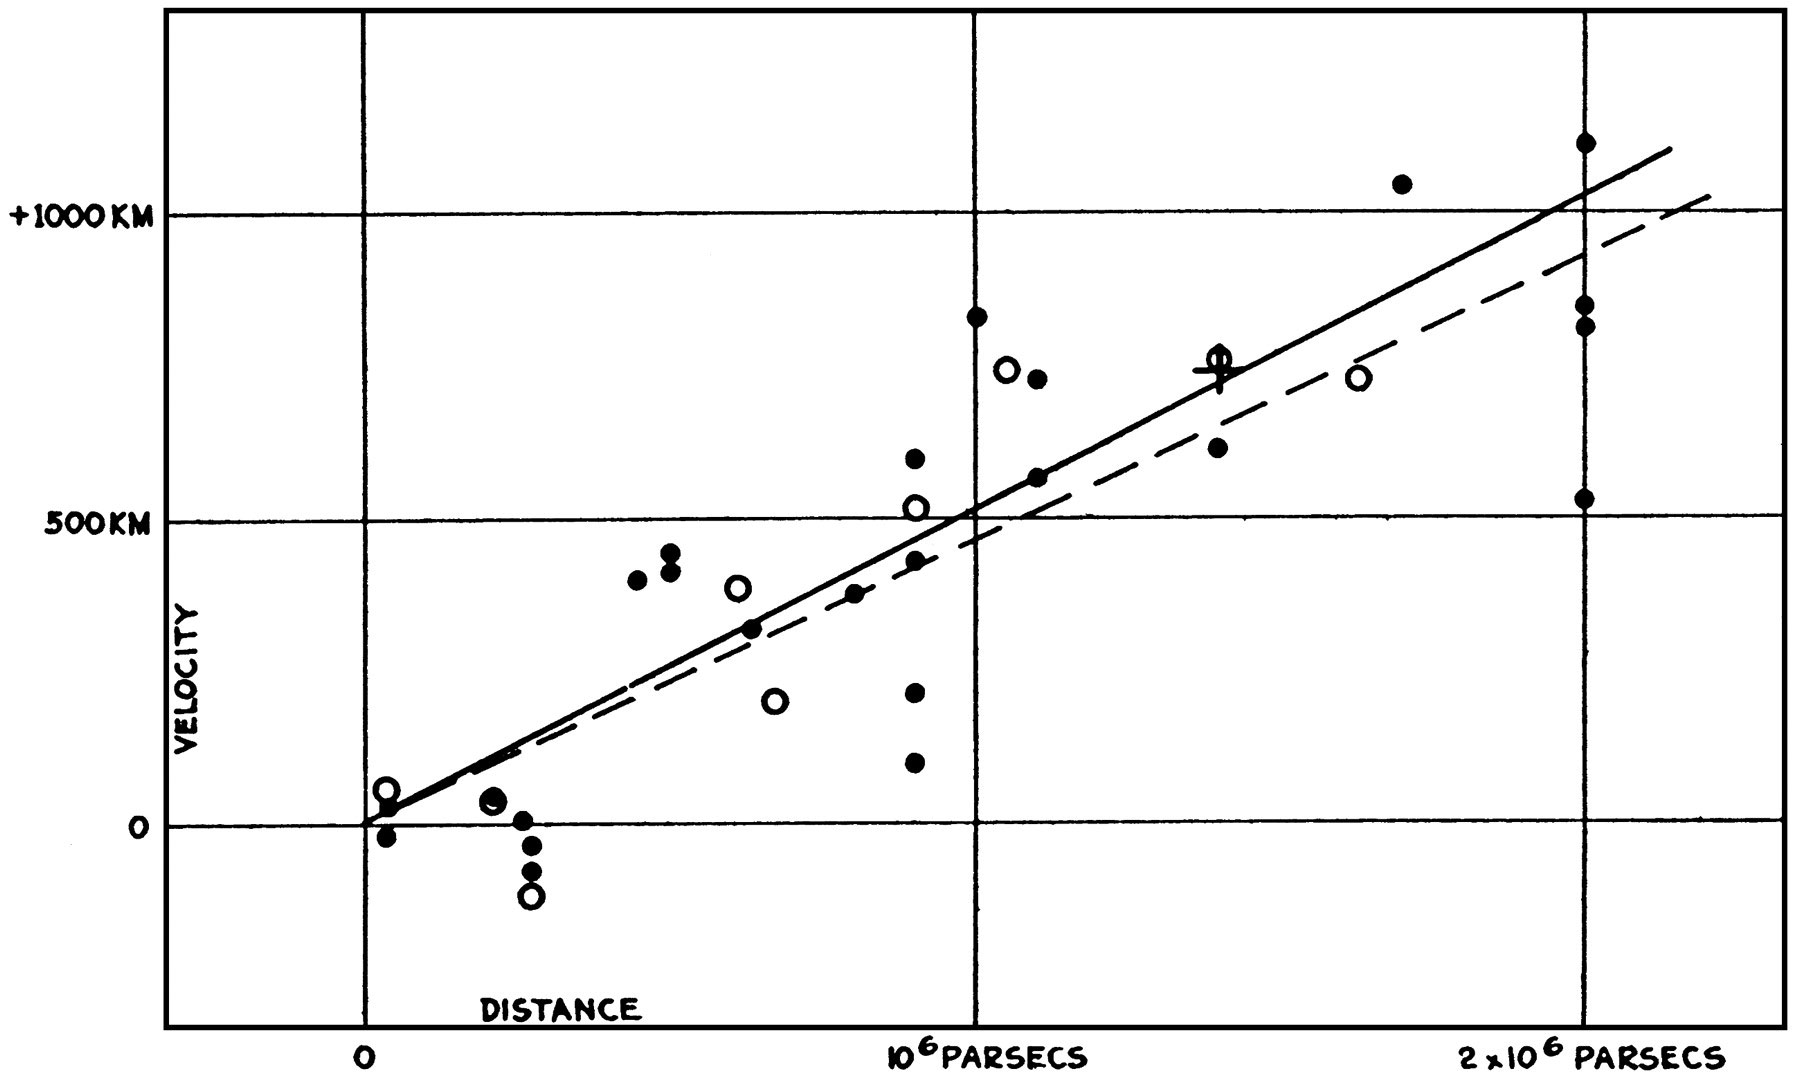
\includegraphics[width=13cm]{1_Introduccion/hubble.jpg}
    \end{center}
    
    \caption{\small Gráfica de una de las publicaciones originales de Hubble. Pone en evidencia que Hubble interpretó el desplazamiento al rojo como debido al efecto Doppler. \comillas{Una Relación entre la Distancia y Velocidad Radial en las Nebulosas Extra-Galácticas}, Los Procesos de la Academia Nacional de Las Ciencias, Volumen 15, Edición 13, 1929: p. 172. ©Huntington Library, San Marino, CA. Fuente: \url{https://www.visionlearning.com/es/library/Proceso-de-la-Ciencia/49/La-Naturaleza-del-Conocimiento-Cient\%c3\%adfico/185}}
    \label{fig:publicacion_hubble}
\end{figure}

Es conveniente aclarar dos puntos. En primer lugar la ley de Hubble no relaciona en realidad velocidades con distancias, sino desplazamientos al rojo con distancias. Esta confusión es debida a que inicialmente el desplazamiento al rojo se achacó a un efecto Doppler tal y como se deduce de las publicaciones originales de Hubble (Figura~\ref{fig:publicacion_hubble}). En segundo lugar, la ley de Hubble no es un modelo físico, es un hecho observable. Actualmente se ha medido del orden de \maths{{10}^{6}} desplazamientos y solo \maths{\sim10} de ellos muestran desplazamientos hacia el azul, siendo estos últimos, todos ellos, objetos del Grupo Local.
Por tanto cualquier interpretación de este fenómeno debe ser coherente con los siguientes puntos:

\vspace{-2mm}
\begin{itemize}
    \item El desplazamiento siempre se produce hacia longitudes de onda mayores, a excepción de los objetos que se encuentran en el Grupo Local.
    \vspace{-2mm}
    
    \item El desplazamiento no depende de la frecuencia, afecta a todo el espectro electromagnético de la misma forma.
    \vspace{-2mm}
    
    \item El desplazamiento es lineal con la distancia al objeto, al menos para el caso de los objetos más próximos, cuya distancia se ha podido determinar por métodos directos.
    \vspace{-2mm}
    
    \item Los desplazamientos son isótropos, es decir, no dependen de la dirección en la que se encuentren en la bóveda celeste, únicamente de la distancia que nos separa de los mismos.
    
\end{itemize}

Además se impone que todas las condiciones anteriores deben cumplirse en cualquier lugar del Universo. Es obvio que no hay evidencia experimental de que esto se cumpla; se trata de una suposición basada en lo que se conoce como principio anti-antropocéntrico, es decir, el observador no se encuentra en un lugar privilegiado. 
Actualmente, la explicación más ampliamente aceptada es la conocida como evolución de la métrica, por ser prácticamente la única explicación disponible. Esta explicación acepta que existe un factor de escala que cambia con el tiempo cosmológico, aumentando la distancia radial que nos separa de los objetos. Dado que la velocidad de la luz es finita y las distancias que nos separan incluso de las galaxias más próximas es enorme, los intervalos de tiempo que tarda la luz en alcanzarnos son lo suficientemente grandes como para que el factor de escala haya cambiado sensiblemente afectando a la longitud de onda de la radiación electromagnética mientras se transmite por el espacio\footnote{Es muy interesante observar que el factor de escala solo afecta al universo a grandes escalas como la distancia entre galaxias. Si el factor de escala afectase a escala de laboratorio de la misma forma que a las escalas astronómicas, cambiaría también nuestros patrones de medida incrementándose en la misma proporción y haciendo indetectable la expansión del universo.}. Los desplazamientos hacia el azul que se observan entre los objetos del Grupo Local se deben a que tienen un movimiento cinemático dirigido hacia nosotros y a que se encuentran relativamente próximos. En este caso, la contribución a $z$ debida al efecto Doppler resulta más importante que la debida a la expansión de la métrica, que siempre contribuye a un desplazamiento al rojo. Para objetos muy lejanos la expansión de la métrica resulta dominante siempre.

A continuación se muestra cómo afecta el cambio del factor de escala a las propiedades de la luz que viaja por el espacio, partiendo de la métrica utilizada en el modelo cosmológico estándar \citep{book:cosmologia}. En un universo en expansión, el \rt\ está directamente relacionado con la distancia.
En el modelo cosmológico estándar de Friedmann-Lema\^{i}tre, las distancias están definidas a partir de la métrica de Robertson-Walker\footnote{Se  demuestra en \cite{book:weinberg_1974} que es la métrica más general que describe un espacio de tetra-dimensional, con tres dimensiones espaciales y una temporal y cuyo subespacio espacial tiene curvatura arbitraria y es maximalmente simétrico.}

\begin{equation}\label{eq:metrica_RW}
    {\mathrm ds}^{2}= {c}^{2}\mathrm dt^2 +{R}^{2}(t) \left( \frac{{\mathrm dr}^{2}}{1-\kappa {r}^{2}} + {r}^{2}\mathrm d{\theta}^{2} +{r}^{2}{\sin}^{2}{\theta}\,\mathrm d{\varphi}^{2} \right),
\end{equation}

siendo \maths{R(t)} el factor de escala, \maths{\kappa} el signo de la curvatura que puede tomar los valores -1, 0 o 1, \textit{t} el tiempo cosmológico y \textit{r}, \maths{\theta} y \maths{\varphi} las coordenadas comóviles expresadas en un sistema de coordenadas esféricas. Debido a la isotropía del espacio, la distancia propia solo depende de la coordenada radial comóvil \maths{r} y es constante con \maths{\theta} y \maths{\varphi}, con lo cual, la métrica se simplifica reduciéndose a

\begin{equation*}
    {\mathrm ds}^{2}= {c}^{2}\mathrm dt^2 +{R}^{2}(t)\;\frac{{\mathrm dr}^{2}}{1-\kappa {r}^{2}}.
\end{equation*}

Supongamos que se emiten dos pulsos de luz. El primero se emite desde un punto coordenada radial comóvil \maths{r=r_e} y tiempo cosmológico \maths{t=t_e}. El segundo con las mismas coordenadas espaciales y un tiempo cosmológico \maths{t_e+T_e}. Estos pulsos se propagan por el espacio durante un tiempo suficientemente grande, como el tiempo necesario para cruzar el espacio entre dos galaxias próximas, tras el cual alcanzan a un observador. El primer pulso lo alcanza en coordenadas \maths{r=0} y \maths{t=t_o}, mientras que el segundo alcanza al observador en \maths{r=0} y \maths{=t_o+T_o}. Teniendo en cuenta que las ondas luminosas viajan por geodésicas (\maths{\mathrm{d}s=0}) y dado que los dos pulsos fueron emitidos y finalmente recibidos en puntos con las mismas coordenadas espaciales, tenemos que:

\begin{equation*}
    \int_{t_e}^{t_0} \frac{\mathrm d t }{R(t)}=\int_{t_e+T_e}^{t_o+T_o} \frac{\mathrm d t }{R(t)}=-{c}^{-1}\int_{r_e}^{0} \frac{\mathrm d r}{\sqrt{1-\kappa {r}^{2}}}.
\end{equation*}

Centraremos la atención en la igualdad establecida por las integrales en las que participa el factor de escala. En principio no podemos realizar las integrales porque desconocemos la función \maths{R(t)}; sin embargo podemos realizar una manipulación sobre los limites de integración:

\begin{align*}
    \int_{t_e+T_e}^{t_o+T_o} \frac{\mathrm d t }{R(t)} =\int_{t_e}^{t_0} \frac{\mathrm d t }{R(t)}\equiv \int_{t_e}^{t_e+ T_e} \frac{\mathrm d t }{R(t)} + \int_{t_e+T_e}^{t_o} \frac{\mathrm d t }{R(t)} \implies \nonumber\\
    \int_{t_e}^{t_e+T_e} \frac{\mathrm d t }{R(t)}= \int_{t_o}^{t_e+ T_e} \frac{\mathrm d t }{R(t)} + \int_{t_e+T_e}^{t_o+T_o} \frac{\mathrm d t }{R(t)} \equiv  \int_{t_o}^{t_o+T_o} \frac{\mathrm d t }{R(t)}. \nonumber \\
\end{align*}

De esta forma, si los tiempos de integración \maths{T_e} y \maths{T_o} han sido mucho más pequeños que el tiempo de propagación de los pulsos por el espacio, el factor de escala puede considerarse constante, teniendo distintos valores cuando los pulsos fueron emitidos y cuando fueron recibidos:

\begin{equation*}
    \frac{1}{R(t_e)}\int_{t_e}^{t_e+T_e} \mathrm d t = \frac{1}{R(t_o)} \int_{t_o}^{t_o + T_o} \mathrm d t \implies \frac{T_e}{R(t_e)}=\frac{T_o}{R(t_o)}.
\end{equation*}

Por comodidad podemos considerar que \maths{T_e} y \maths{T_o} son los periodos de la onda luminosa cuando fue emitida y cuando fue observada, respectivamente. Utilizando la ecuación \maths{T=\lambda/c} y la definición general de corrimiento al rojo (Ec. \ref{eq:z_general}) obtenemos que

\begin{equation}\label{eq:metrica_vs_z}
    \frac{R(t_o)}{R(t_e)}=\frac{\lambda_o}{\lambda_e}=1+z.
\end{equation}

El desplazamiento al rojo no se debe por tanto a un efecto Doppler, si no porque el incremento del factor de escala, afecta de la misma forma a la longitud de onda de la radiación electromagnética durante el tiempo de propagación que a las distancias propias.

Desarrollando en serie de Taylor el inverso del factor de escala en torno a \maths{t=t_o},

\begin{align}
    z =\frac{R(t_o)}{R(t_e)}-1 & = \frac{\dot{R}(t_o)}{R(t_o)}(t_o-t)+\left[ {\left(\frac{\dot{R}(t_o)}{R(t_o)}\right)}^{2}-\frac{1}{2}\frac{\ddot{R}(t_o)}{R(t_o)}\right]{(t_o-t)}^{2} +\cdots \nonumber
\end{align}

podemos recuperar la ley de Hubble al identificar el término \maths{\dot{R}(t_o)/R(t_o)} con el valor de la  constante de Hubble en el tiempo cosmológico actual \maths{H_o} y truncándolo en el término de segundo orden

\vspace{-3mm}
 
\begin{align}
    z={H}_{o}(t_o-t)+{H}_{o}^{2}\left[1+\frac{1}{2} {q}_{o} \right]{(t_o-t)}^{2} +\cdots .\nonumber
\end{align}

La ley de Hubble en el contexto del modelo estándar debe considerarse como una aproximación a la Ecuación \ref{eq:metrica_vs_z} \citep{book:cosmologia}.

\subsection{Técnicas para determinar el desplazamiento al rojo.}

En este trabajo estaremos haciendo referencia continuamente a \comillas{\rt\ espectroscópicos} y \comillas{\rt\ fotométricos}. Esos nombres hacen referencia a la técnica con la que se obtuvo esa medida. A continuación se explicará brevemente en que consisten estas técnicas. Cabe mencionar que el método propuesto en la Sección \ref{sec:3_redshift_hatlas} de esta memoria forma parte de las técnicas fotométricas.

\subsubsection{\anglicismo{Redshift} espectroscópico.}

Cuando se habla de \rt\ espectroscópico nos estamos refiriendo a una técnica para determinar el \rt\ de los objetos celestes. El \rt\ espectroscópico consiste en identificar algunas de las líneas espectrales de absorción o emisión de algún elemento químico en la luz proveniente de un objeto celeste y comparar la longitud de onda a la que se encuentran con la que debería tener si proviniesen de una muestra en reposo. Este es el primer método que se utilizó para determinar el desplazamiento al rojo de los objetos celestes y permite determinar el \rt\ de forma muy precisa; el problema que tiene es que requiere de largos tiempos de exposición (\maths{\sim3} horas en un telescopio de 4 m para un objeto de magnitud aparente \maths{\sim22}) y aunque existen técnicas para obtener varios espectros simultáneamente, es imposible hacerlo de un número grande de objetos en un tiempo razonable \citep{tesis:robert_juncosa}.

\subsubsection{\anglicismo{Redshift} fotométrico.}

Se trata de otra técnica para determinar el \rt. En este caso se utilizan varios filtros espectrales que permiten el paso de luz en una determinada región electromagnética muy estrecha. Después se utiliza una base de datos donde se almacena una colección de las SEDs de varios modelos de galaxias y se obtiene un espacio de parámetros (\rt, tipo espectral, magnitud, flujo...) que permite el mejor ajuste posible entre las medidas y los modelos. Estas técnicas se conocen con el nombre genérico de SED-\anglicismo{fitting procedure}. 

Estos métodos surgen con la aparición de las cámaras de gran campo y los cartografiados (\anglicismo{surveys}) con los que es posible cubrir grandes áreas de cielo con tiempos de exposición más cortos que en el caso espectroscópico. Tienen la ventaja de ser mucho más rápidos que las técnicas espectroscópicas ya que como hemos dicho que obtener el espectro de cada objeto de un cartografiado es un trabajo muy lento. Como desventaja cabe señalar que la medida resultante tiene una mayor imprecisión que el método anterior. Además se hace necesario tener una base de datos lo suficientemente amplia (que represente a los objetos que se estén estudiando) con la que comparar y cobertura fotométrica amplia. Aún en ese caso, siempre puede haber objetos que tengan sus propias singularidades espectrales y por tanto sean difíciles de clasificar. En cuanto a las medidas es importante la cobertura espectral y la precisión fotométrica.
Un factor limitante para la aplicación de este método suele ser que la cobertura espectral disponible para un determinado objeto suele ser pequeña, es decir, no se dispone de un número significativo de medidas sobre una región suficientemente amplia del espectro electromagnético; como es imposible disponer de un único aparato que realice medidas en todo el espectro electromagnético, puede ser necesario disponer de varios instrumentos. 

Los errores asociados a estas medidas dependen significativamente tanto del algoritmo utilizado, como del intervalo de \maths{z} al que pertenece la medida. Por ese motivo, lo que se suele hacer es comparar las medidas espectroscópicas y fotométricas disponibles sobre una población suficientemente grande de objetos y se estima el error a partir de las dispersión de estas diferencias. Formalmente se calcula \maths{\sigma=\sqrt{{\langle \left({z_{\mathrm{phot}}-z_{\mathrm{spec}}}\right)}^{2}\rangle}} (siendo \maths{z_{\mathrm{spec}}} el \rt\ espectroscópico y \maths{z_{\mathrm{phot}}} el fotométrico) para cada uno de los objetos; después se obtiene un valor promedio mediante un ajuste. La dispersión típica que se suele obtener mediante estos métodos es \maths{\sigma \simeq 0.1\times (1+z)} \citep{tesis:robert_juncosa}. En el caso concreto de ANNZ,\footnote{ Se trata de un paquete de software, disponible de forma gratuita, para la estimación del \rt\ fotométrico utilizando redes neuronales artificiales (de ahí el nombre ANNZ, \anglicismo{Artificial Neural Networks}).} muestra una dispersión media cuadrática de \maths{\sigma=0.023} al aplicarlo sobre los objetos del SDSS 1 (\anglicismo{Sloan~Digital~Sky~Survey~Data~Release} 1), en el rango de \maths{0\lesssim z\lesssim0.7} \citep{article:annz}.

\subsection{Lentes gravitatorias}

Se denomina lente gravitatoria a los efectos que produce la gravedad sobre la luz, en particular la desviación de la trayectoria de luz procedente de objetos los objetos fuente debido a la presencia de objetos muy masivos llamados lente.
El fenómeno que se produce varía dependiendo de la masa y forma del objeto lente y la posición relativa entre la fuente, la lente y el observador. Típicamente las lentes gravitatorias se clasifican en dos tipos, en base únicamente a los efectos cuantitativos que producen; las \comillas{lentes gravitatorias débiles} producen magnificaciones débiles (magnificación\footnote{Es suficiente interpretar este valor cómo el incremento del brillo de la fuente por efecto de la lente gravitatoria. La definición formal de la magnificación es complicada y no tiene cabida en este trabajo (para una explicación extensa se puede consultar \citealt{book:encyclopedia}).} \maths{\mu<2}) y distorsiones moderadas, mientras que las \comillas{lentes gravitatorias fuertes}, producen magnificaciones más intensas (\maths{\mu \sim2} o más) y pueden producir imágenes múltiples muy distorsionadas de un mismo objeto. Al depender sus efectos de factores geométricos y gravedad, no vienen mezclados con otros fenómenos físicos, lo cual hace de las lentes un fenómeno particularmente interesante para estudiar, por ejemplo, distribuciones de materia oscura.
También es reseñable que la distorsión actúa  por igual sobre todo el espectro electromagnético, por lo cual las lentes gravitatorias carecen de aberración cromática.

El estudio de los efectos que produce la gravedad sobre la luz puede resultar una tarea muy complicada, por ello es común recurrir a una serie aproximaciones; generalmente se llevan a cabo las siguientes:

\begin{itemize}
    \item Campos gravitatorios suficientemente débiles\footnote{La distinción entre lentes gravitatorias débiles y fuertes no depende de la intensidad del campo gravitatorio.}, en los que las partículas con masa siguen la dinámica newtoniana.
    
    \item La extensión de la masa de la lente a lo largo del eje de observación es despreciable en comparación con la distancia entre la fuente-lente y lente-observador (aproximación de lente delgada).
    
    \item  La lente y la fuente se encuentran aproximadamente en la línea de observación, de forma que la separación angular entre ambos, \maths{ \theta \simeq  \sin{(\theta)} }.
    
    \item Los efectos de difracción son despreciables, porque incluso la longitud de onda de las ondas de radio, es demasiado pequeña frente a las escalas de los elementos que forman la lente gravitatoria típica.
    
\end{itemize}

Consideremos un haz de luz en presencia de punto\footnote{Si la masa que se interpone tiene una distribución de masa con simetría esférica, la luz fuera de la distribución es desviada como si se tratase de un objeto puntual (ley de Gauss).} de masa \maths{M} a una distancia \maths{R} perpendicular a él. Teniendo en cuenta las aproximaciones anteriores, el efecto debido a la gravedad sobre los fotones es que estos se desvían un ángulo \maths{\theta} hacia la masa puntual,

\begin{equation}\label{eq:bending_angle}
    \theta=\frac{4 GM}{{c}^{2}R}
\end{equation}

donde \maths{G} es la constante de gravitación universal y \maths{c} la velocidad de la luz. Para campos gravitatorios débiles, la aproximación se aplica siempre que \maths{R \gg \frac{2 GM}{{c}^{2}}\equiv{r}_{s}} (radio de Schwarzschild, \maths{{r}_{s}}, que se corresponde con el radio aparente del horizonte de sucesos en un agujero negro). Para el caso de la masa típica de una estrella (\masassolares{M\sim 1}), \maths{{r}_{s}\sim 10\:\mathrm{km}}, para la masa típica de una galaxia (\masassolares{M\sim {10}^{11}}) \maths{{r}_{s}<1\:\mathrm{pc}}, mientras que para un cúmulo de galaxias (\masassolares{M\sim {10}^{13}}) \maths{{r}_{s}< {10}^{3}\:\mathrm{pc}}, por lo que en astronomía esta condición se cumple fácilmente \citep{book:encyclopedia}.
La medida del ángulo de desviación de la luz procedente de una estrella debido a la masa del Sol es considerado como el primer test de la teoría de la Relatividad General. La Ecuación \ref{eq:bending_angle} predice el valor correcto; en contraste con la dinámica de Newton que predice la mitad de ese valor.

Las lentes gravitatorias debidas a estrellas que se encuentran en la Vía Láctea, se da en una de cada \maths{{10}^{6}} estrellas, por lo que resultan un fenómeno raro si se compara con en número de lentes gravitatorias producidas por las galaxias y cuásares que se produce aproximadamente en uno de cada \maths{{10}^{3}} \citep{book:encyclopedia}. 

\subsubsection{Radio de Einstein.}

Se considerará ahora el caso particular en el que la fuente y la masa que hace de lente se encuentran exactamente sobre la línea de visión.

\begin{figure}[htb]
    \begin{center}
         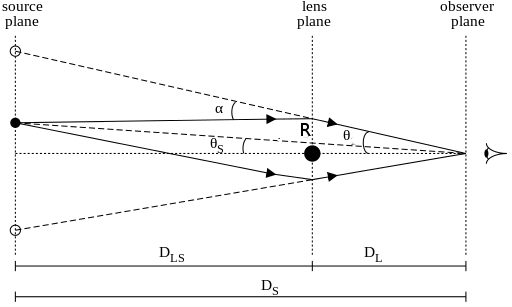
\includegraphics[width=14cm]{1_Introduccion/Gravitational_lens_geometry.png}
    \end{center}
    \caption{\small {Distribución geométrica de los elementos que conforman una lente gravitatoria.} (Fuente: \url{https://en.wikipedia.org/wiki/Einstein_radius\#/media/File:Gravitational_lens_geometry.svg})}
    \label{fig:lente}
\end{figure}

\newpage

Para realizar el estudio utilizaremos la expresión \ref{eq:bending_angle} junto con argumentos geométricos basados en la Figura \ref{fig:lente}. A partir del dibujo

\begin{equation*}
    D_S\; \theta= D_S\;{\theta}_{S} + {D}_{LS}\;\alpha,
\end{equation*}

que podemos reescribir despejando $\alpha$: 

\begin{equation}\label{eq:alpha_geometrica}
    \alpha =(\theta -{\theta}_{S})\frac{{D}_{S}}{{D}_{LS}}.
\end{equation}

La distancia entre el haz luminoso y la fuente puntual es \maths{R}. Si \maths{R} es suficientemente pequeño en comparación con \maths{D_L}, se puede realizar la aproximación

\begin{equation*}
    \frac{R}{{D}_{L}} = \sin{\theta} \approx \theta \implies R \approx \theta D_L
\end{equation*}

y el ángulo de desviación de los fotones debido a la masa gravitatoria será:

\begin{equation}\label{eq:alpha_gravitatoria}
    \alpha =\frac{4 GM}{{c}^{2}\theta {D}_{L}}.
\end{equation}

El último paso consiste en igualar la Ecuación \ref{eq:alpha_geometrica} y la Ecuación \ref{eq:alpha_gravitatoria}:

\begin{equation*}
     \frac{4 GM}{{c}^{2}\theta {D}_{L}}=(\theta -{\theta}_{S})\frac{{D}_{S}}{{D}_{LS}}
\end{equation*}

y notar que para el caso en que la masa se encuentra justo detrás de la lente, \maths{{\theta}_{S}=0}; el ángulo \maths{\theta} recibe entonces el nombre de radio de Einstein, que se denota mediante \maths{{\theta}_{E}},

\begin{equation}\label{eq:radio_einstein}
    {{\theta}_{E}}^{2}=\frac{4 GM}{{c}^{2} }\frac{D_{LS}}{D_{L} D_{S}}.
\end{equation}

Este caso particular de lente gravitatoria da lugar al fenómeno conocido como anillos de Einstein, en la que la imagen de la fuente forma un circulo centrado en el objeto lente. Los anillos de Einstein han sido detectados en varias ocasiones, pero son un fenómeno muy difícil de observar ya que los requisitos necesarios para que tengan lugar son muy improbables. Sin embargo, el concepto es importante, porque los fenómenos asociados a lentes gravitatorias fuertes se producen a escalas de \maths{{\theta}_{E}}.
Cuando \maths{D_S\gg D_L} entonces se cumple también \maths{D_S\simeq D_{LS}} y la Ecuación \ref{eq:radio_einstein} se suele aproximar como

\begin{equation}\label{eq:radio_einstein_magnitud}
    {\theta}_{E} \simeq 0.1 \times { {\left( \frac{M\;\mathrm{en}\;M_{\odot}}{D_L \;\mathrm{en\;pc}}\right)} }^{1/2}\;\mathrm{en\;arcsec},
\end{equation}

que es más adecuada para hacer cálculos teniendo en cuenta las unidades más utilizadas en astrofísica \citep{book:encyclopedia}.

\newpage

\subsection{Inferencia bayesiana.}

La inferencia bayesiana es un método racional para la actualización de creencias. Se trata de un método de razonamiento aproximado, es decir, no se considera que una determinada información sea cierta o falsa con carácter absoluto; en su lugar, se parte de una hipótesis inicial a la que se le asigna un número como medida de la credibilidad que se tiene sobre la misma y con cada nueva observación se calcula de nuevo el factor numérico con el que se cuantifica el credibilidad de la hipótesis. La herramienta matemática que se utiliza para la actualización de creencias es el Teorema de Bayes.

\subsubsection{Teorema de Bayes y teorema de las probabilidades totales.}

Uno de los conceptos fundamentales en inferencia bayesiana es el concepto de probabilidad condicional. La probabilidad condicional, es la probabilidad de que ocurra un suceso \maths{A}, dado que también tiene lugar otro suceso \maths{B}. La probabilidad condicional se escribe \maths{P(A|B)} y se lee «\resalta{probabilidad de \maths{A} dado \maths{B}}».

\begin{definition}[Probabilidad condicional]
Sean dos sucesos A y B tales que la la probabilidad de que ocurra B no sea nula, P(B)>0, se define la probabilidad de A dado B como

\begin{equation}\label{eq:prob_condicional}
    P(A|B)=\frac{P(A \cap B)}{P(B)},
\end{equation}

siendo \maths{P(A \cap B)} la probabilidad conjunta de los dos sucesos, o dicho de otra forma, la probabilidad de que se den los dos sucesos simultáneamente.

\end{definition}

A partir de la definición de probabilidad condicional podemos escribir que

\begin{equation*}
    P(A \cap B)=P(A|B)P(B)=P(B|A)P(A).
\end{equation*}

Si los sucesos son independientes entre si, \maths{P(A|B) \equiv P(A)} y \maths{P(B|A) \equiv P(B)},
y por tanto la probabilidad de ocurrencia de ambos sucesos de forma simultanea es igual al producto de la probabilidad de ocurrencia de los sucesos de forma independiente, esto es,

\begin{equation*}
    P(A \cap B)=P(A)P(B).
\end{equation*}

En el caso de que los sucesos no sean independientes, la probabilidad de que tenga lugar \maths{A} dado \maths{B} será:

\begin{equation*}
    P(A|B)=\frac{P(B|A) P(A)}{P(B)},
\end{equation*}

que es lo que se llama \textit{Teorema de Bayes\footnote{El teorema de Bayes es un resultado incontrovertible partiendo de la definición de probabilidad condicional y los axiomas de Kolmogórov.} para los sucesos A y B}.

\begin{theorem}[Teorema de Bayes]
Sea \maths{\Omega} un conjunto de sucesos %espacio muestral
compuesto por un conjunto \maths{n} de particiones mutuamente excluyentes\footnote{Tanto el Teorema de Bayes como el Teorema de la probabilidad total, son también válidos cuando existe un conjunto infinito numerable de causas disjuntas dos a dos.} ( \maths{\Omega=\{H_1,H_2,H_3...H_n\}},  \maths{H_i \cap H_j=\emptyset} siendo \maths{i\neq j}) y sea B un suceso tal que \maths{B\subset \Omega}, la probabilidad de que el suceso \maths{B} sea consecuencia de \maths{H_{i}} viene dada por

\begin{equation}\label{eq:teorema_bayes}
    P(H_i|B)=\frac{P(B|H_i)\;P(H_i)}{P(B)},
\end{equation}

donde el divisor \maths{P(B)} representa la probabilidad de que tenga lugar el suceso \maths{B}.
\end{theorem}

\begin{theorem}[Teorema de la Probabilidad Total]

Sea \maths{\Omega} un conjunto de sucesos compuesto por un conjunto \maths{n} de particiones mutuamente excluyentes  ( \maths{\Omega=\{H_1,H_2,H_3...H_n\}},  \maths{H_i \cap H_j=\emptyset} siendo \maths{i\neq j}) y sea \maths{B\subset \Omega} un suceso cualquiera del que se conocen las probabilidades condicionales \maths{P(B|H_{i})},  entonces la probabilidad del suceso \maths{B} viene dada por

\begin{equation}
    P(B)=\sum_{i=1}^{n}{P(B|H_i)P(H_i)}.
\end{equation}

\end{theorem}

\begin{figure}[htb]
    \begin{center}
         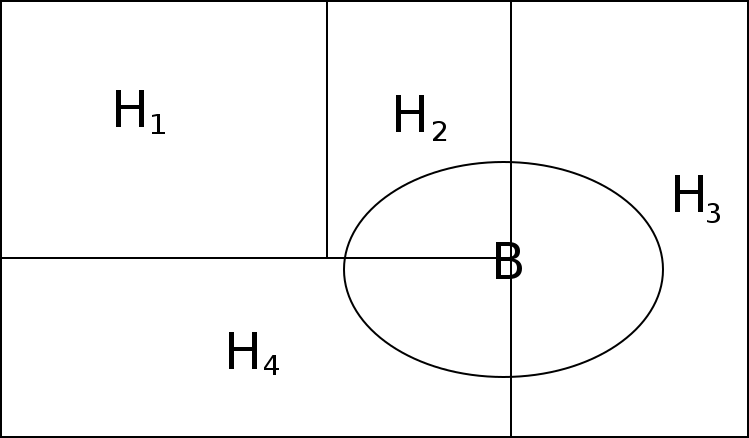
\includegraphics[width=14cm]{1_Introduccion/conjuntos.png}
    \end{center}
    \caption{\small Representación de un espacio muestral \maths{\Omega} de área unidad, constituido por cuatro particiones mutuamente excluyentes, ( \maths{\Omega=\{H_1,H_2,H_3,H_4\}},  \maths{H_i \cap H_j=\emptyset} siendo \maths{i\neq j}). En esta representación un conjunto de suceso \maths{B} equivale a una región del espacio muestral con una forma y una superficie características.} 
    
    \label{fig:conjuntos}
\end{figure}

Tanto el Teorema de Bayes como el Teorema de la Probabilidad Total admiten una interpretación gráfica. El espacio muestral \maths{\Omega} puede representarse por una superficie de área unidad, donde cada subconjunto \maths{X} tiene una probabilidad de ocurrir igual al área que ocupa  \maths{P(X)}, (Figura \ref{fig:conjuntos}). Las probabilidades condicionales se representan por las regiones que forman parte simultáneamente de dos subconjuntos del espacio muestral. En la Figura~\ref{fig:conjuntos}, el subconjunto \maths{B} es el único que solapa con otros subconjuntos. Las áreas de las regiones de \maths{B} que forman parte de uno de los subconjuntos \maths{H_i} vienen representadas por \maths{P(B|H_i)P(H_i)}, que es equivalente al área del subconjunto \maths{H_i} que forma parte de \maths{B} y que viene representado por \maths{P(H_i|B)P(B)}.

\newpage

\subsubsection{El factor de Bayes}

Supongamos que disponemos de un conjunto de datos \maths{D=\{x_1,x_2 \dots x_n\}} y dos hipótesis alterativas \maths{H_1} y \maths{H_2} para las que suponemos la función verosimilitud \maths{p(D|H_1)} y \maths{p(D|H_2)} y una \resalta{probabilidad a priori} \maths{p(H_1)} y \maths{p(H_2)}. Debido a la evidencia de los datos, se produce una trasformación de la \resalta{probabilidad a priori} en \resalta{probabilidad a posteriori} \maths{p(H_{k}|D)} a través del teorema de Bayes,

\begin{equation*}
    p(H_{k}|D)=\frac{p(D|H_{k})p(H_{k})}{p(D)}=\frac{p(D|H_{k})p(H_{k})}{p(D|H_{1})p(H_1)+p(D|H_2)p(H_2)}\qquad \qquad \qquad (k=1,2)
\end{equation*}

donde el subíndice \maths{k} indica de qué hipótesis se trata. Para elegir cuál de las dos es la hipótesis es más verosímil, se realiza el cociente de la \resalta{probabilidad a posteriori} de cada hipótesis,

\begin{equation*}
   \frac{p(H_{1}|D)}{p(H_2|D)}=\frac{p(D|H_{1})}{p(D|H_2)}\frac{p(H_{1})}{p(H_2)}.
\end{equation*}

Al cociente

\begin{equation*}
    B_{12}=\frac{p(D|H_1)}{p(D|H_2)}
\end{equation*}

se le denomina factor de Bayes.

\begin{definition}[Factor de Bayes]\label{def:factor_bayes}
El factor de Bayes se define como el cociente de la función verosimilitud de dos hipótesis alternativas

\begin{equation}\label{eq:factor_bayes}
    B_{12}=\frac{p(D|H_1)}{p(D|H_2)},
\end{equation}

donde los subíndices hacen referencia a la hipótesis 1 y 2 respectivamente.
\end{definition}


Si el valor de \maths{B_{12}} es superior a la unidad, el valor de \maths{p(D|H_1)} es superior al de \maths{p(D|H_2)} y la confianza sobre \maths{H_1} es mayor que sobre \maths{H_2}. En caso de ser inferior a la unidad, los datos refuerzan la confianza de \maths{H_2} sobre \maths{H_1}. En adelante, tomaremos los valores de la Tabla \ref{tab:bayes_interpretacion} como escala referencia.


\begin{table}[h]
\renewcommand\tablename{Tabla}
\renewcommand{\arraystretch}{1.5}
\centering
    
    \setlength{\extrarowheight}{-2pt}
    \begin{tabular}{ C{4cm} C{4cm} C{5cm} }
        \hline
        ${B}_{12}$	& $\log_{10}{(B_{12})}$	& Confianza sobre $H_1$ \\
        %\cline{1-3}
        \hline
        \hline
    \end{tabular}

    \setlength{\extrarowheight}{-1mm}
    \begin{tabular}{ C{4cm} C{4cm} C{5cm} }
        <1 &  <0 &  $H_1$ es refutada \\
        1 --- 3.2 &  0 --- $\frac{1}{2}$ &   Débil  \\
        3.2 --- 10 &  $\frac{1}{2}$ --- 1 &   Sustancial  \\
        10 --- 31.6 &  1 --- $\frac{3}{2}$ &   Fuerte  \\
        31.6 --- 100 &  $\frac{3}{2}$ --- 2 & Muy fuerte  \\
        >100 &  >2 &   Absoluta  \\


        \hline
    \end{tabular}

    \caption{\small Escala de referencia que nos relaciona el valor del factor de Bayes con la confianza que tenemos sobre la hipótesis \maths{H_1}. Se trata de la tabla de referencia utilizada por Harold Jeffreys en 1961 (consultar~\citealt{article:Robert_E_Kass_1995}).}

    \label{tab:bayes_interpretacion}
\end{table}

\newpage

En el caso particular del método de \cross\ que se va a utilizar en este trabajo, lo que pretendemos es contrastar la hipótesis \maths{H_1} de que los emparejados considerados están formados por observaciones de un mismo objeto astronómico frente a la hipótesis \maths{H_2} de que se trata de observaciones pertenecientes a dos objetos diferentes.

Si las medidas de un parámetro pertenecen a un único objeto astronómico la función densidad de probabilidad conjunta \maths{p(D|\theta,H_k)} se obtiene mediante el producto de las funciones densidad de probabilidad asociadas para cada medida \maths{p_i(x_i|\theta,H_k)} que representan la probabilidad de que una medida \maths{x_i} se corresponda exactamente con su verdadero valor \maths{\theta} y la función verosimilitud para \maths{H_1} resulta ser

\begin{equation}
    p(D|H_1)=\int p(\theta|H_1)p(D|\theta,H_1)\,d\theta=\int p(\theta|H_1)\prod_{i=1}^{n}p_i(x_i|\theta,H_1)\,d\theta,
\end{equation}

siendo \maths{p(\theta|H_1)} la densidad de \resalta{probabilidad a priori} de la hipótesis \maths{H_1}. Para el caso de la hipótesis \maths{H_2} las medidas \maths{x_i} pertenecen a distintos valores verdaderos \maths{\theta_i} por lo que la función verosimilitud de \maths{H_2} se calcula como

\begin{equation}
    p(D|H_2)=\prod_{i=1}^{n}\left[\int p({\theta}_i|H_2)p_i(x_i|{\theta}_i,H_2)\,d\theta_i \right].
\end{equation}

En los casos en que disponemos de \maths{q} conjuntos de medidas \maths{D_s} diferentes, asociados a lo distintos parámetros, dispondremos de \maths{q} factores de Bayes. Suponiendo cada uno de los parámetros que hemos elegido son igualmente válidos para determinar la verosimilitud de nuestras hipótesis, el factor de Bayes conjunto se obtiene como el producto de los factores de Bayes asociados a cada parámetro,

\begin{equation}\label{eq:bayes_multiple}
    B_{12}=B^{1}_{12}\times B^{2}_{12} \dots B^{q}_{12}=\prod_{s=1}^{q}\frac{p(D_{s}|H_1)}{p(D_{s}|H_2)}.
\end{equation}

De esta manera, cada nueva observación cambia el conjunto de valores \maths{D_s} lo que cambia la verosimilitud de cada hipótesis y en consecuencia el factor de Bayes. En esto consiste la actualización de creencias basada en el razonamiento bayesiano.